

\documentclass[11pt,a4paper,twoside]{article}

\usepackage[utf8]{inputenc}
\usepackage[english]{babel} 
\usepackage{notoccite}
\usepackage[skip=0.5\baselineskip]{caption}
\hyphenation{GTKWave}
\usepackage{listings}
\usepackage[all]{nowidow}
\usepackage{amsmath} %Matrix package
\usepackage{csvsimple} %csv reading package
\usepackage{authblk} %author information
\usepackage{caption}
\usepackage{multicol}


\usepackage{graphicx}
\graphicspath{{./}{../../figlib/}{../mat/}{../sim/}}
\def\FontLn{% 16 pt normal
  \usefont{T1}{phv}{m}{n}\fontsize{16pt}{16pt}\selectfont}
\def\FontLb{% 16 pt bold
  \usefont{T1}{phv}{b}{n}\fontsize{16pt}{16pt}\selectfont}
\def\FontMn{% 14 pt normal
  \usefont{T1}{phv}{m}{n}\fontsize{14pt}{14pt}\selectfont}
\def\FontMb{% 14 pt bold
  \usefont{T1}{phv}{b}{n}\fontsize{14pt}{14pt}\selectfont}
\def\FontSn{% 12 pt normal
  \usefont{T1}{phv}{m}{n}\fontsize{12pt}{12pt}\selectfont}

\renewcommand{\rmdefault}{phv}
\renewcommand{\sfdefault}{phv}
\usepackage{geometry}	
\geometry{verbose,tmargin=2.5cm,bmargin=2.5cm,lmargin=2.5cm,rmargin=2.5cm}

%\usepackage{setspace}
%\renewcommand{\baselinestretch}{1.5}

\usepackage[pdftex]{hyperref} % enhance documents that are to be
                              % output as HTML and PDF
\hypersetup{colorlinks,       % color text of links and anchors,
                              % eliminates borders around links
%            linkcolor=red,    % color for normal internal links
            linkcolor=black,  % color for normal internal links
            anchorcolor=black,% color for anchor text
%            citecolor=green,  % color for bibliographical citations
            citecolor=black,  % color for bibliographical citations
%            filecolor=magenta,% color for URLs which open local files
            filecolor=black,  % color for URLs which open local files
%            menucolor=red,    % color for Acrobat menu items
            menucolor=black,  % color for Acrobat menu items
%            pagecolor=red,    % color for links to other pages
            pagecolor=black,  % color for links to other pages
%            urlcolor=cyan,    % color for linked URLs
            urlcolor=black,   % color for linked URLs
	          bookmarks=true,         % create PDF bookmarks
	          bookmarksopen=false,    % don't expand bookmarks
	          bookmarksnumbered=true, % number bookmarks
	          pdftitle={report},
            pdfauthor={Andre C. Marta},
%            pdfsubject={Thesis Title},
%            pdfkeywords={Thesis Keywords},
            pdfstartview=FitV,
            pdfdisplaydoctitle=true}

\usepackage[numbers,sort&compress]{natbib} % <<<<< References in numbered list [1],[2],...
\usepackage{subcaption} 
\usepackage{mdframed}

%%%%%%%%%%%%%%%%%%%%%%%%%%%%%%%%%%%%%%%%%%%%%%%%%%%%%%%%%%%%%%%%%%%%%%%%
%     Begin Document                                                   %
%%%%%%%%%%%%%%%%%%%%%%%%%%%%%%%%%%%%%%%%%%%%%%%%%%%%%%%%%%%%%%%%%%%%%%%%


\begin{document}

% Set plain page style (no headers, footer with centered page number)
\pagestyle{plain}

% Set roman numbering (i,ii,...) before the start of chapters
%\pagenumbering{roman}

% ----------------------------------------------------------------------
%  Cover page
% ----------------------------------------------------------------------
\begin{titlepage}
%%%%%%%%%%%%%%%%%%%%%%%%%%%%%%%%%%%%%%%%%%%%%%%%%%%%%%%%%%%%%%%%%%%%%%%%
%                                                                      %
%     File: frontvover.tex                                      %
%     Tex Master: report.tex                                           %
%                                                                      %
%     Author: Group 41                                           %
%     Last modified :  3 Mar 2021                                      %
%                                                                      %
%%%%%%%%%%%%%%%%%%%%%%%%%%%%%%%%%%%%%%%%%%%%%%%%%%%%%%%%%%%%%%%%%%%%%%%%

\thispagestyle {empty}

% IST Logo - Signature A
% parameters: bb=llx lly urx ury (bounding box), width=h_length, height=v_length, angle=angle, scale=factor, clip=true/false, draft=true/false. 
\includegraphics[bb=9.5cm 11cm 0cm 0cm,scale=0.29]{IST_A_CMYK_POS}

\begin{center}
%

\vspace{1.0cm}


% Title, author and degree
\vspace{1cm}
{\FontLb Circuit Theory and Electronics Fundamentals} \\ % <<<<< EDIT TITLE
\vspace{1cm}
{\FontSn Aerospace Engineering, Técnico, University of Lisbon} \\ % <<<<< EDIT COURSE
\vspace{1cm}
{\FontSn T1 Laboratory Report} \\
\vspace{1cm}
{\FontSn March 6, 2021} \\ % <<<<< EDIT DATE (corresponds to date of oral examination)
\vspace{1cm}
\author{Duarte Brito 96373 \and Henrique Caraça 96393 \and Nuno Ribeiro 96459}
\end{center}


\end{titlepage}

% ----------------------------------------------------------------------
% Dedication page (optional)
% ----------------------------------------------------------------------
%\input{dedication} 
%\cleardoublepage

% ----------------------------------------------------------------------
%  Acknowledgments (optional)
% ----------------------------------------------------------------------
%\input{acknowledgements}
%\cleardoublepage

% ----------------------------------------------------------------------
%  Abstract (both in English and Portuguese)
% ----------------------------------------------------------------------
%\input{resumo} 
%\cleardoublepage

%\input{abstract} 

% ----------------------------------------------------------------------
%  Table of contents, list of tables, list of figures and nomenclature
% ----------------------------------------------------------------------

% Table of contents
%
\tableofcontents

% List of tables
%\addcontentsline{toc}{section}{\listtablename}
%\listoftables
%\cleardoublepage 

% List of figures
%\addcontentsline{toc}{section}{\listfigurename}
%\listoffigures
%\cleardoublepage 

% Set arabic numbering (1,2,...) after preface
%
%\setcounter{page}{1}
%\pagenumbering{arabic}

% ----------------------------------------------------------------------
%  Body
% ----------------------------------------------------------------------

\section{Introduction}
\label{sec:introduction}

\indent

% state the learning objective 
The objective of this laboratory assignment is to make a Bandpass filter using an OP-AMP.

The equivalent circuit can be seen in Figure~\ref{fig:circuit}. 

This circuit is made up of an amplifier (an OP-AMP and resistors $R_3$ and $R_4$), a high pass filter (the left part, that is $C_1$ and $R_1$),  and a low pass filter (the right part, that is $R_2$ and $C_2$) .

In Section~\ref{sec:simulation analysis}, the circuit is analysed by
means of a ngspice simulation. In Section~\ref{sec:theoretical analysis}, a theoretical analysis of the circuit is
presented. The results are then compared in Section~\ref{sec:theoretical analysis}. The conclusions of this study are outlined in Section~\ref{sec:conclusion}.



\begin{figure}[h!] \centering
	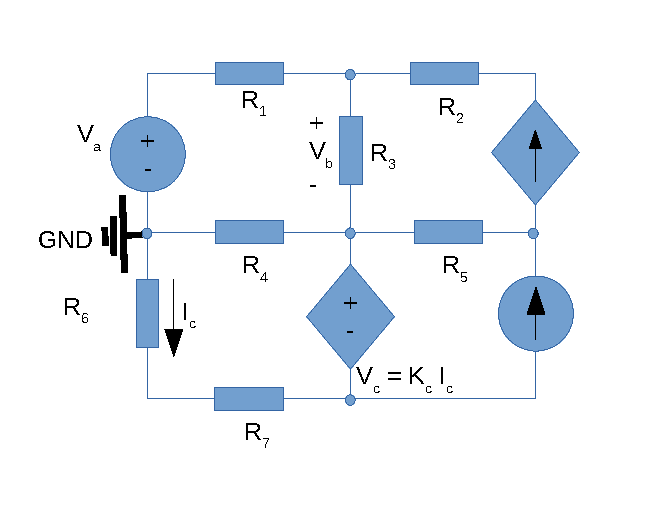
\includegraphics[width=0.6\linewidth]{circ.pdf}
	\caption{Used Circuit.}
	\label{fig:circuit}
\end{figure}







\section{Theoretical Analysis}
\label{sec:theoretical analysis}
%%%%%%%%%%%%%%%%%%%%%%%%%%%%%%%%%%%%%%%%%%%%%

\subsection{Voltage rectifier}
First the current resulting from the transformer, which is considered ideal is calculated using the formula $V_2/n_2=V_1/n_1 $, thereupon, the circuit is analyzed to understand which diodes from the rectifier are on and off for each signal of current. Next, by using KVL, it is possible to define the tension on the capacitor without addressing its discharge $V_c=A cos(w.t)-(n_{diodes} \cdot V_{on}) $, being A the amplitude of the voltage after being transformed in the inductor. 

\subsection{Envelope detector}

\textbf{Capacitor discharge:}
By using KCL, it is possible to write that $i_d = i_c + i_r$ ($i_r$ being the current if the equivalent resistor of voltage regulator).
Once the capacitor is charged and because there is fluctuation due to the sinusoidal nature of the voltage coming from the rectifier, there will be a point where $i_r = -i_c$. At this point, the diodo will turn off and the capacitor will begin to discharge. This point is called $t_{off}$ and it can be calculated like $$ t_{off}=(1/w)\cdot atan(1/w/(C  \cdot  R_{v_{reg}})).$$The function that defines the discharging is calculated using a formula obtained in the lectures: $$ V_{exp}=(A-2.V_{on}).cos(w \cdot t_{off})exp(-(t-t_{off})/(CR_{v_{reg}})$$



%\begin{figure}[h!]
 %  \includegraphics[width=.5\columnwidth]{circ_inf_0.pdf}
  %  \centering
   % \caption{Circuit at t$<$0} 
    %\label{t<0}
%\end{figure}

\subsection{Voltage at the Capacitor}

The voltage at the capacitor will be the maximum between the sinusoidal function coming from the voltage rectifier and the function of the discharge.

We can decompose this voltage, $v_C$, in its DC component, $V_c$, and its AC component, $v_c$ ($V_c$ is the mean of the function and $v_c$ is the function minus $V_c$).


\subsection{Voltage Regulator}

\textbf{Output Voltage:}
The output voltage, $v_O$, will be the voltage measured in the nodes of the first and last nodes.
This voltage can be decomposed in two components: $$v_O = V_o + v_o$$

$V_o $ will be equal to number of diodos, $n_d$ times $V_{on}$.

To get $v_o$, it is used the incremental model of the diodo, where it can be replaced by a resistor $r_d$.
After using voltage dividir, one can get the following:
$$ v_o = \frac{n_d \cdot r_d}{n_d \cdot r_d + R} \cdot v_s$$

After doing this, the output voltage, $v_O$, has been calculated.





\subsection{Results and Comparisons}



The results obtained in the simulation and theoretical analysis were similar (as it can be seen in the graphics bellow):

\begin{itemize}
  \item The value of the voltage drop of the envelope detector is close
  \item The ripple's order of magnitude is the same
  \item The value of M is similar
\end{itemize}

Note that the DC component of the voltage regulator in the theoretical analysis is equal to the one obtained in the simulation because the value of $V_{on}$ used in the theoretical analysis was taken from NGSpice. 

\begin{figure}[h]
    \centering
\subfloat[Simulation Results]{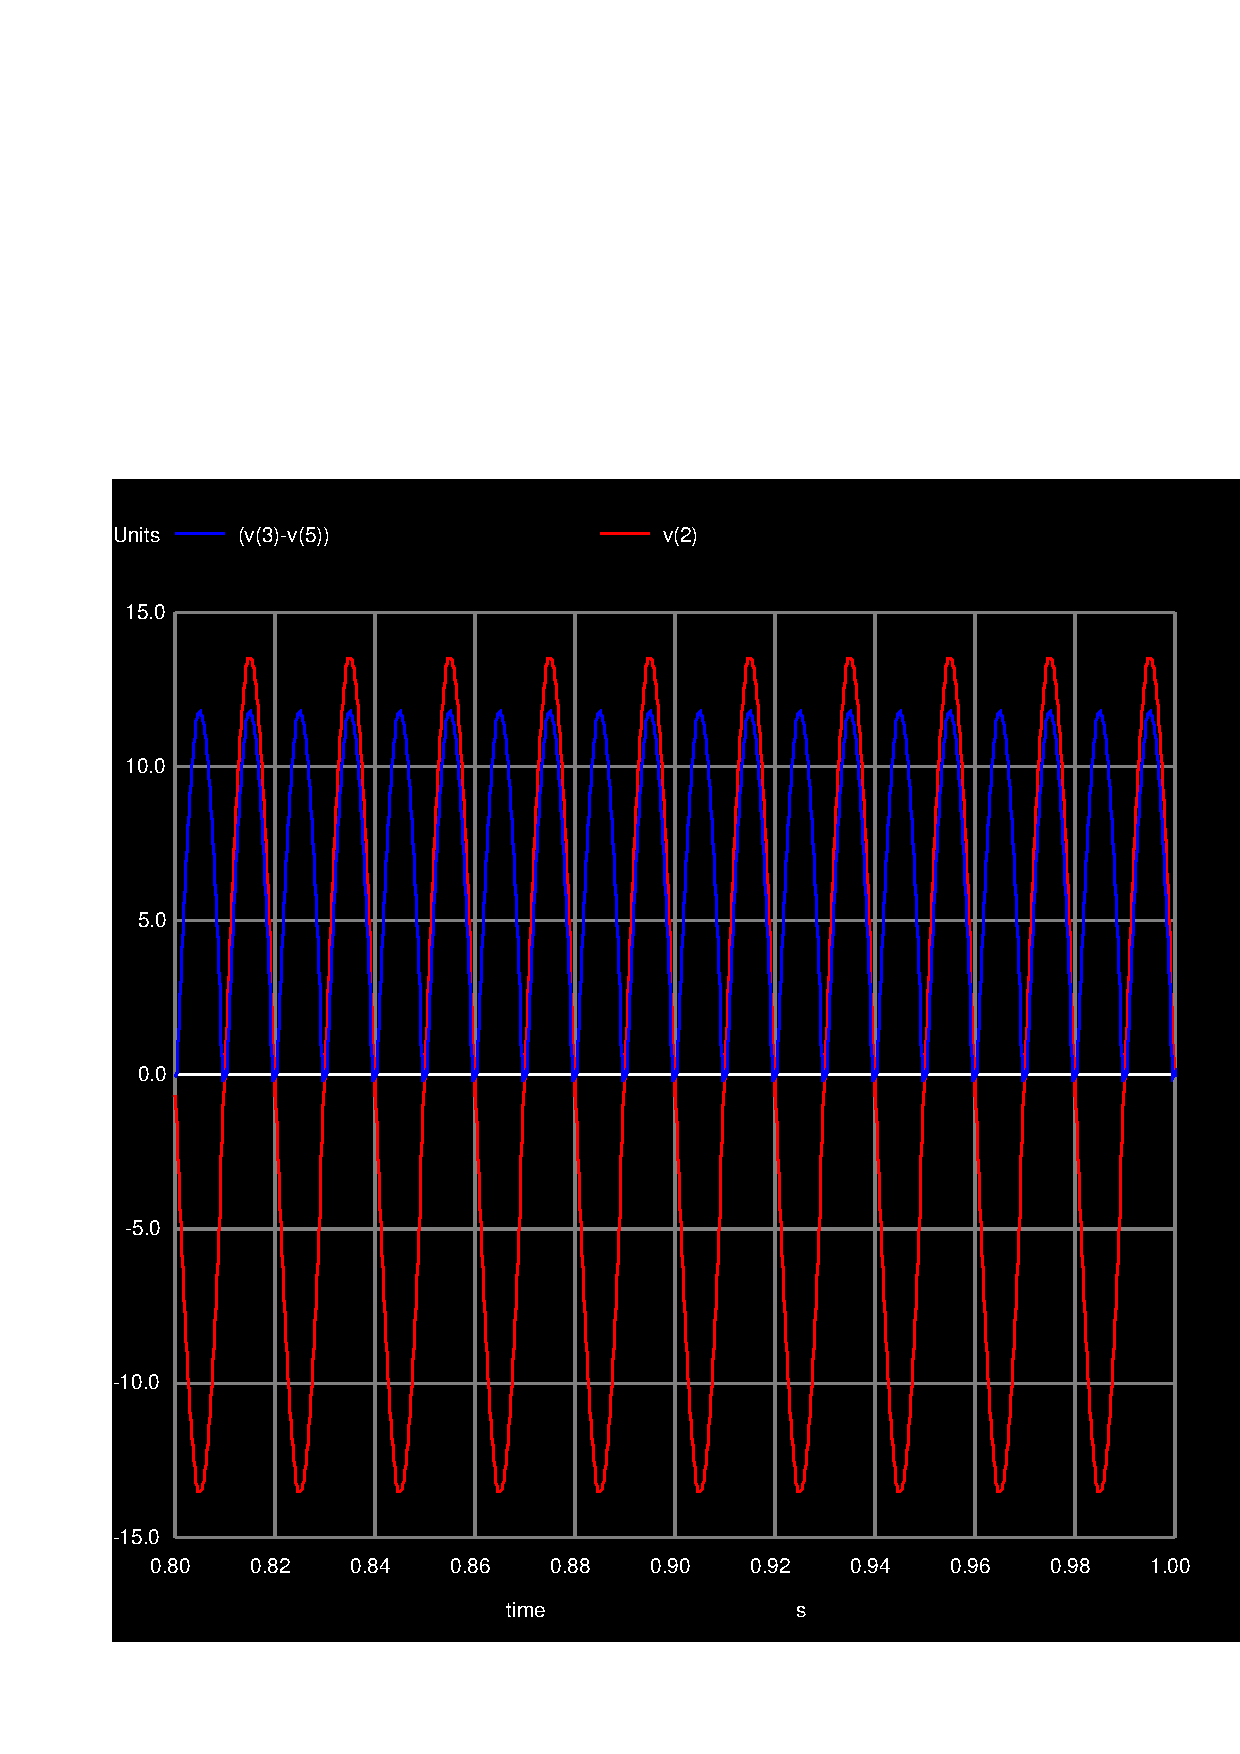
\includegraphics[width=0.40\textwidth]{../sim/outputvoltage.pdf}
\label{Fig_2_estatica}}
  \hfill
\subfloat[Theoretical Results]{\includegraphics[width=0.55\textwidth]{../mat/results_2.png}
\label{Fig_2_dinamica}}
\end{figure}

  \begin{figure}[h]
     \centering
     \caption{Envelope Detector and Voltage Regulator}
     \label{fig_2_reação_normal}
 \end{figure}


\begin{figure}[h]
    \centering
\subfloat[Simulation Results]{\includegraphics[width=0.40\textwidth]{../sim/zoom2.pdf}
\label{Fig_2_estatica}}
  \hfill
\subfloat[Theoretical Results]{\includegraphics[width=0.55\textwidth]{../mat/results.png}
\label{Fig_2_dinamica}}
\end{figure}

  \begin{figure}[h]
     \centering
     \caption{Deviation from the objective of 12 V}
     \label{fig_2_reação_normal}
 \end{figure}


\begin{table}[h]
  \centering
  \begin{tabular}{|l|r|}
    \hline    
    %{\bf Name} & {\bf Value [A or V]} \\ \hline
    \input{../sim/info}
  \end{tabular}
  \caption{Spice results. The M value and the cost were calculated by an additional octave script included in the git.}
  \label{tab:info}
\end{table}

\begin{table}[h]
  \centering
  \begin{tabular}{|l|r|}
    \hline    
    %{\bf Name} & {\bf Value [A or V]} \\ \hline
    Parameter & Value \\
\hline
Output DC level & 11.998660 V \\
\hline
Ripple & 0.009528 V \\
\hline
Cost & 64.815017 MU \\
\hline
M & 1.884083 \\
\hline

  \end{tabular}
  \caption{Spice results. The M value and the cost were calculated by an additional octave script included in the git.}
  \label{tab:info}
\end{table}




\section{Simulation Analysis}
\label{sec:simulation}

\subsection{Operating Point Analysis}

Table~\ref{tab:op} shows the simulated operating point results for the circuit
under analysis. Compared to the theoretical analysis results, one notices the
following differences: describe and explain the differences.

\begin{table}[h]
  \centering
  \begin{tabular}{|l|r|}
    \hline    
    {\bf Name} & {\bf Value [A or V]} \\ \hline
    @gb[i] & -2.47520e-04\\ \hline
@id[current] & 1.005321e-03\\ \hline
@r1[i] & 2.364560e-04\\ \hline
@r2[i] & -2.47520e-04\\ \hline
@r3[i] & -1.10640e-05\\ \hline
@r4[i] & 1.201119e-03\\ \hline
@r5[i] & -1.25284e-03\\ \hline
@r6[i] & 9.646630e-04\\ \hline
@r7[i] & 9.646630e-04\\ \hline
v(1) & 5.076387e+00\\ \hline
v(2) & 4.828240e+00\\ \hline
v(3) & 4.317615e+00\\ \hline
v(4) & 4.862301e+00\\ \hline
v(5) & 8.665725e+00\\ \hline
v(6) & -1.94693e+00\\ \hline
v(7) & -2.95363e+00\\ \hline
v(9) & -1.94693e+00\\ \hline

  \end{tabular}
  \caption{Operating point. A variable preceded by @ is of type {\em current}
    and expressed in Ampere; other variables are of type {\it voltage} and expressed in
    Volt.}
  \label{tab:op}
\end{table}

\lipsum[1-1]


\subsection{Transient Analysis}

Figure~\ref{fig:trans} shows the simulated transient analysis results for the
circuit under analysis. Compared to the theoretical analysis results, one
notices the following differences: describe and explain the differences.

\begin{figure}[h] \centering
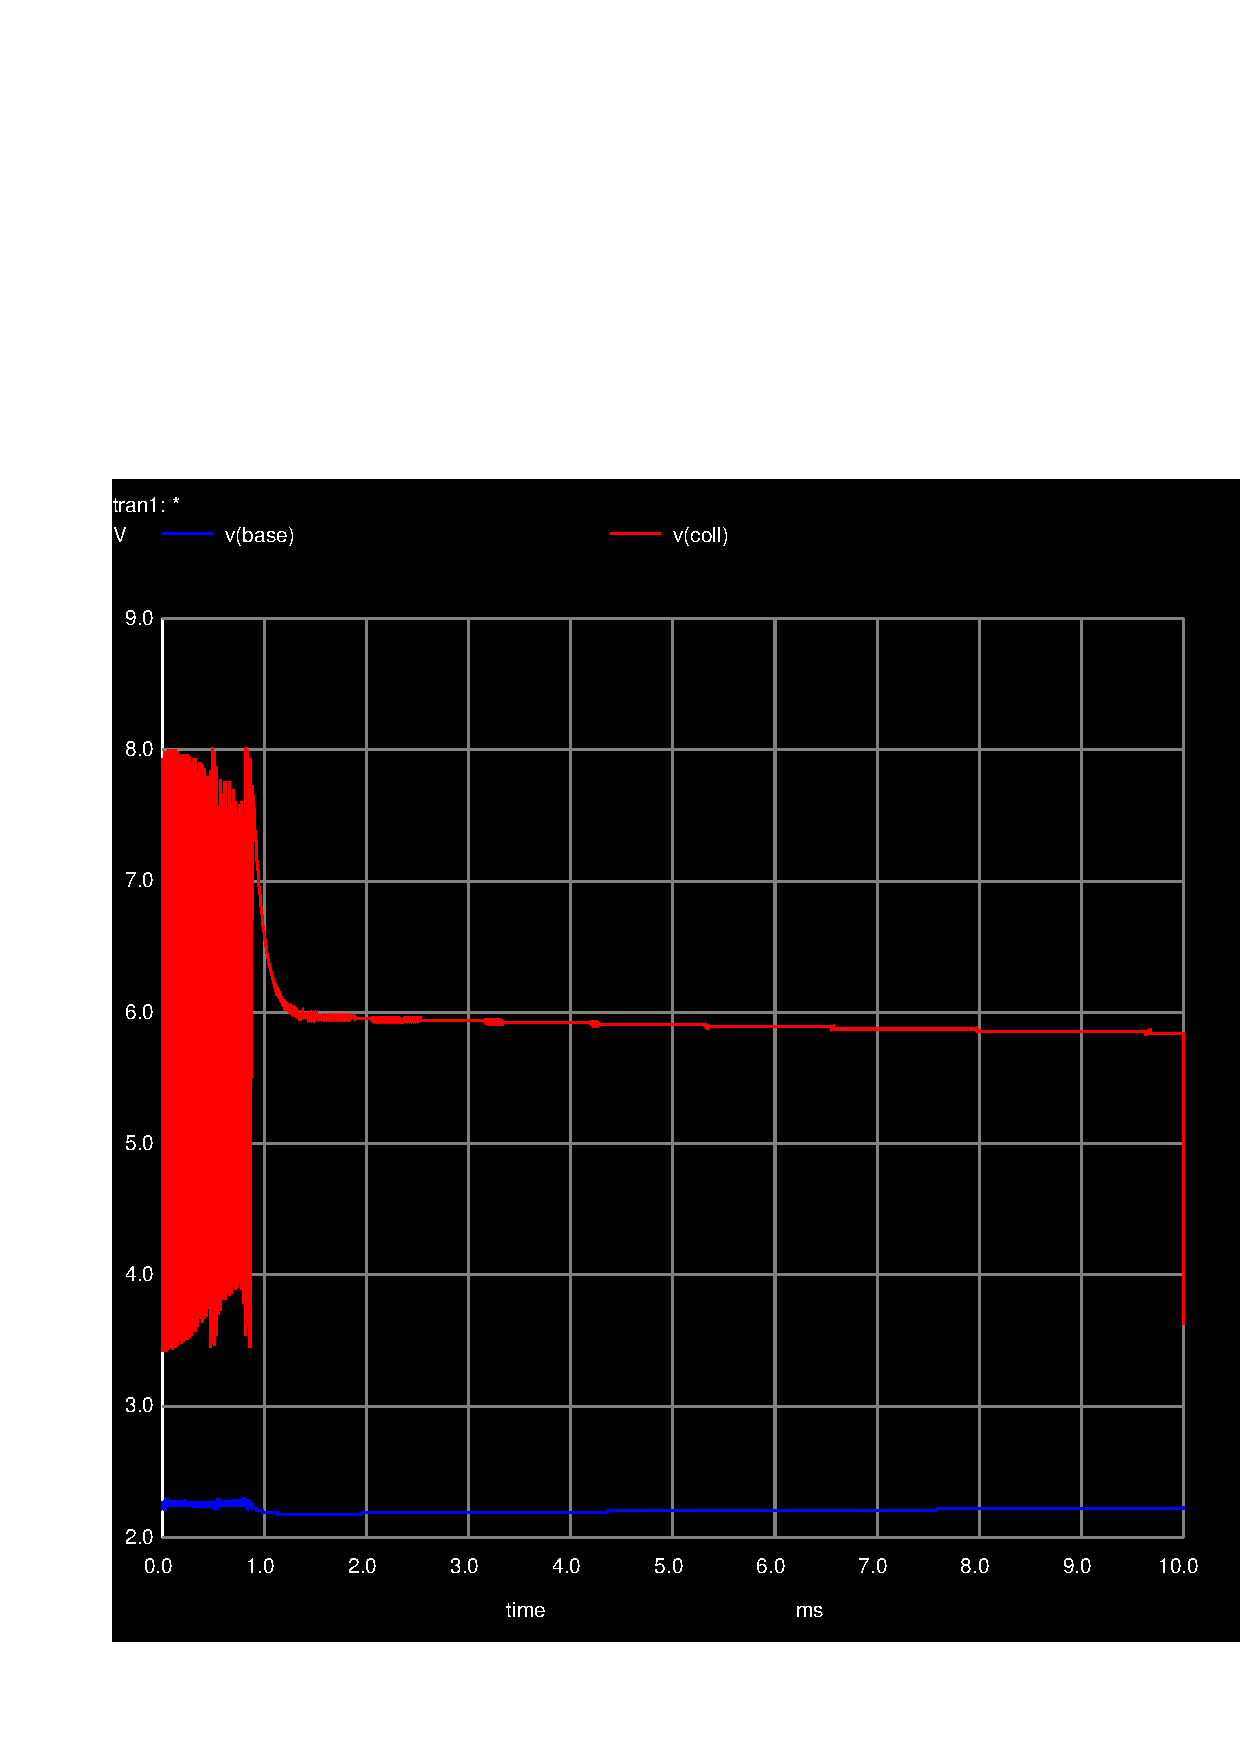
\includegraphics[width=0.6\linewidth]{trans.pdf}
\caption{Transient output voltage}
\label{fig:trans}
\end{figure}

\lipsum[1-1]



\subsection{Frequency Analysis}

\subsubsection{Magnitude Response}

Figure~\ref{fig:acm} shows the magnitude of the frequency response for the
circuit under analysis. Compared to the theoretical analysis results, one
notices the following differences: describe and explain the differences.

\begin{figure}[h] \centering
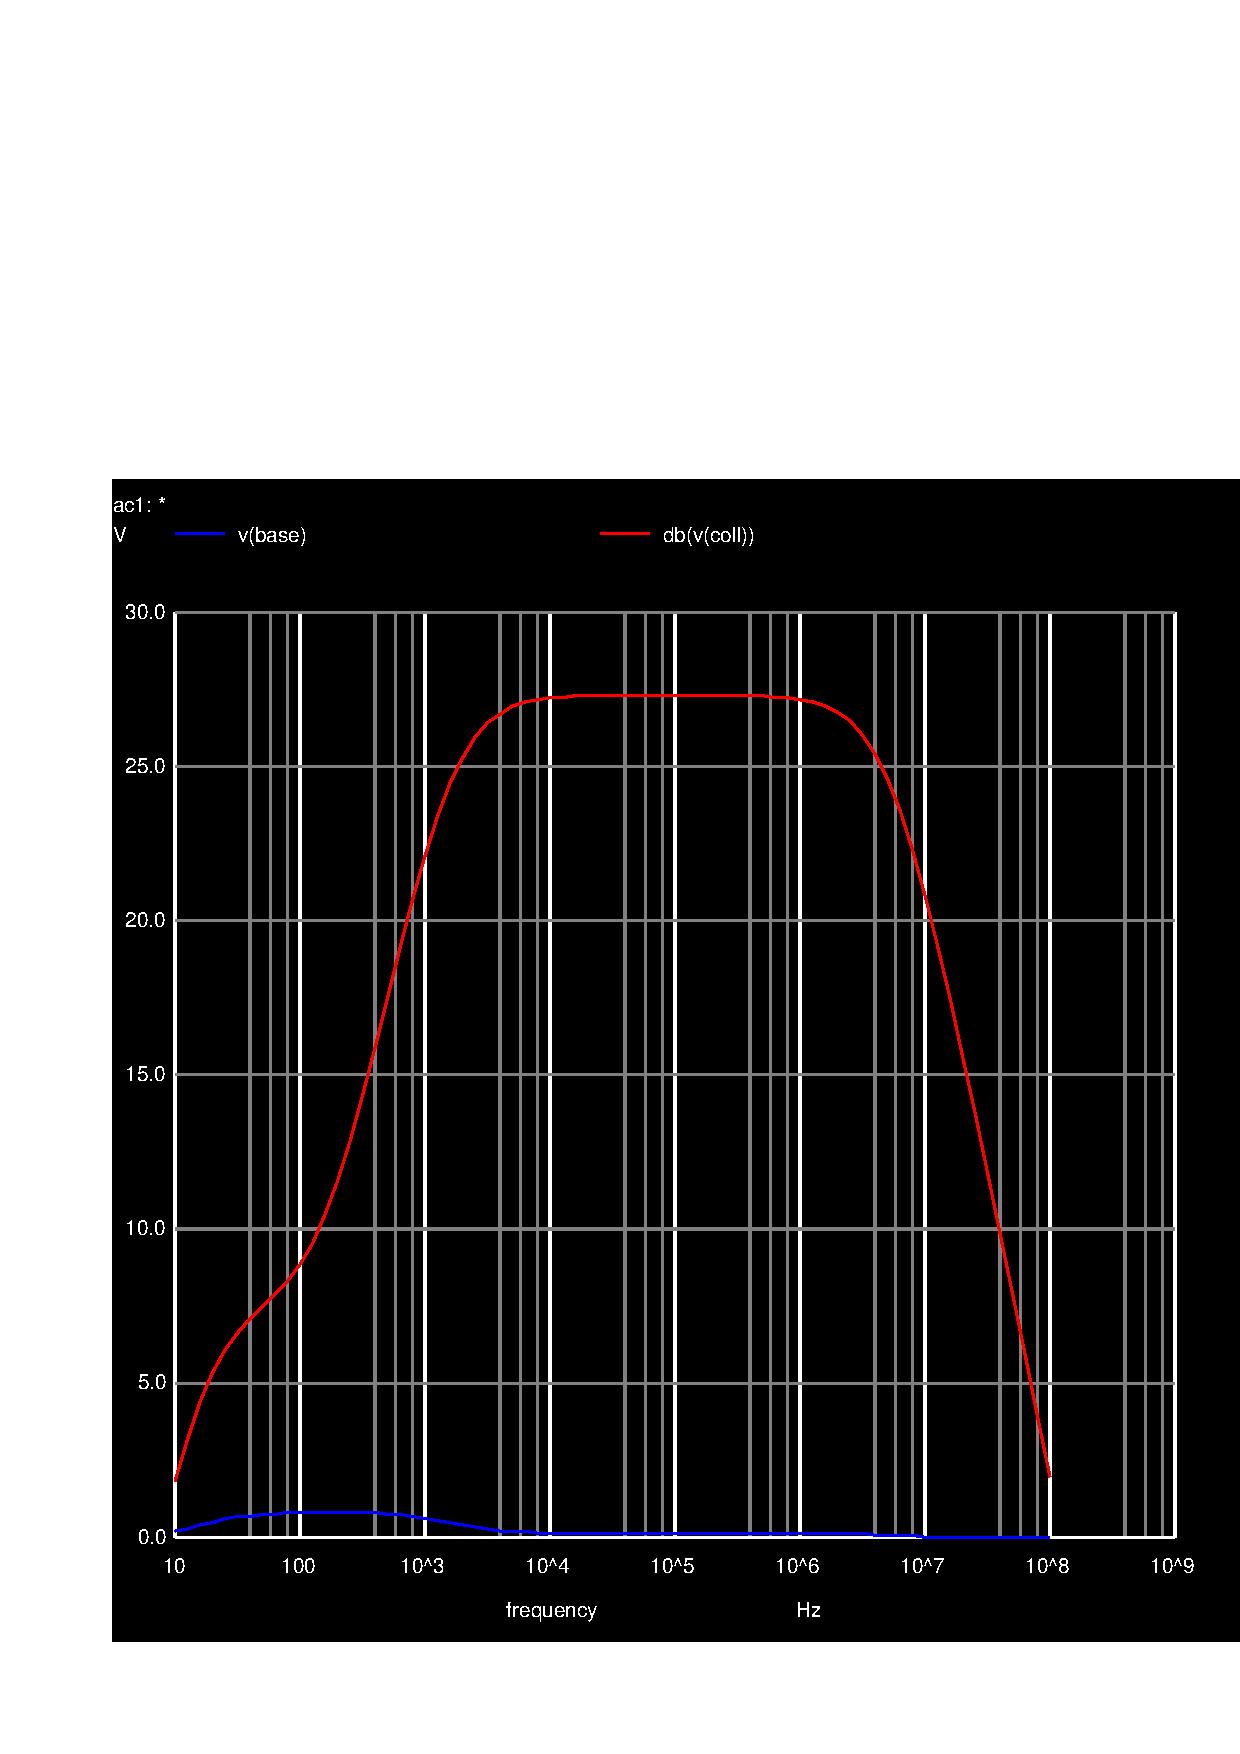
\includegraphics[width=0.6\linewidth]{acm.pdf}
\caption{Magnitude response}
\label{fig:acm}
\end{figure}

\lipsum[1-1]

\subsubsection{Phase Response}

Figure~\ref{fig:acp} shows the magnitude of the frequency response for the
circuit under analysis. Compared to the theoretical analysis results, one
notices the following differences: describe and explain the differences.

\begin{figure}[h] \centering
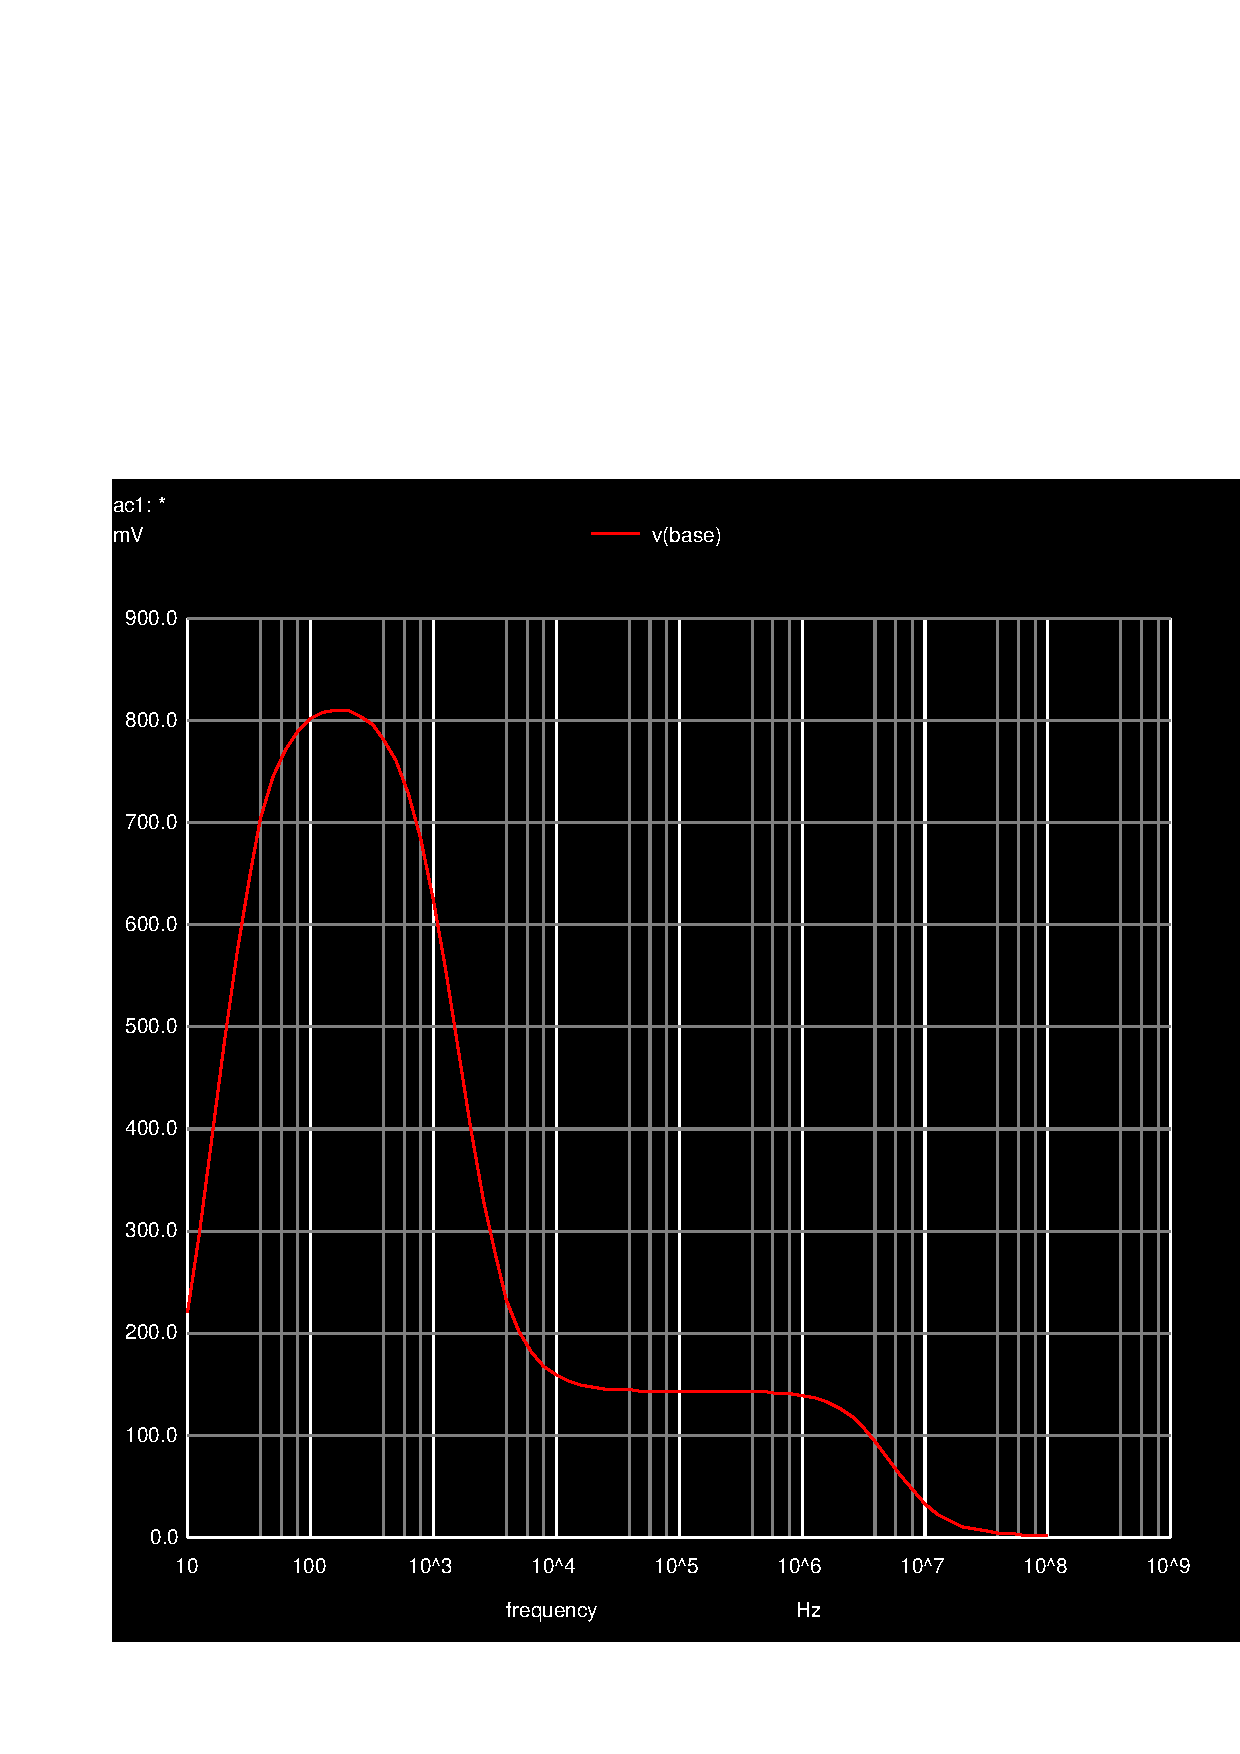
\includegraphics[width=0.6\linewidth]{acp.pdf}
\caption{Phase response}
\label{fig:acp}
\end{figure}

\lipsum[1-1]

\subsubsection{Input Impedance}

Figure~\ref{fig:zim} shows the magnitude of the frequency response for the
circuit under analysis. Compared to the theoretical analysis results, one
notices the following differences: describe and explain the differences.

\begin{figure}[h] \centering
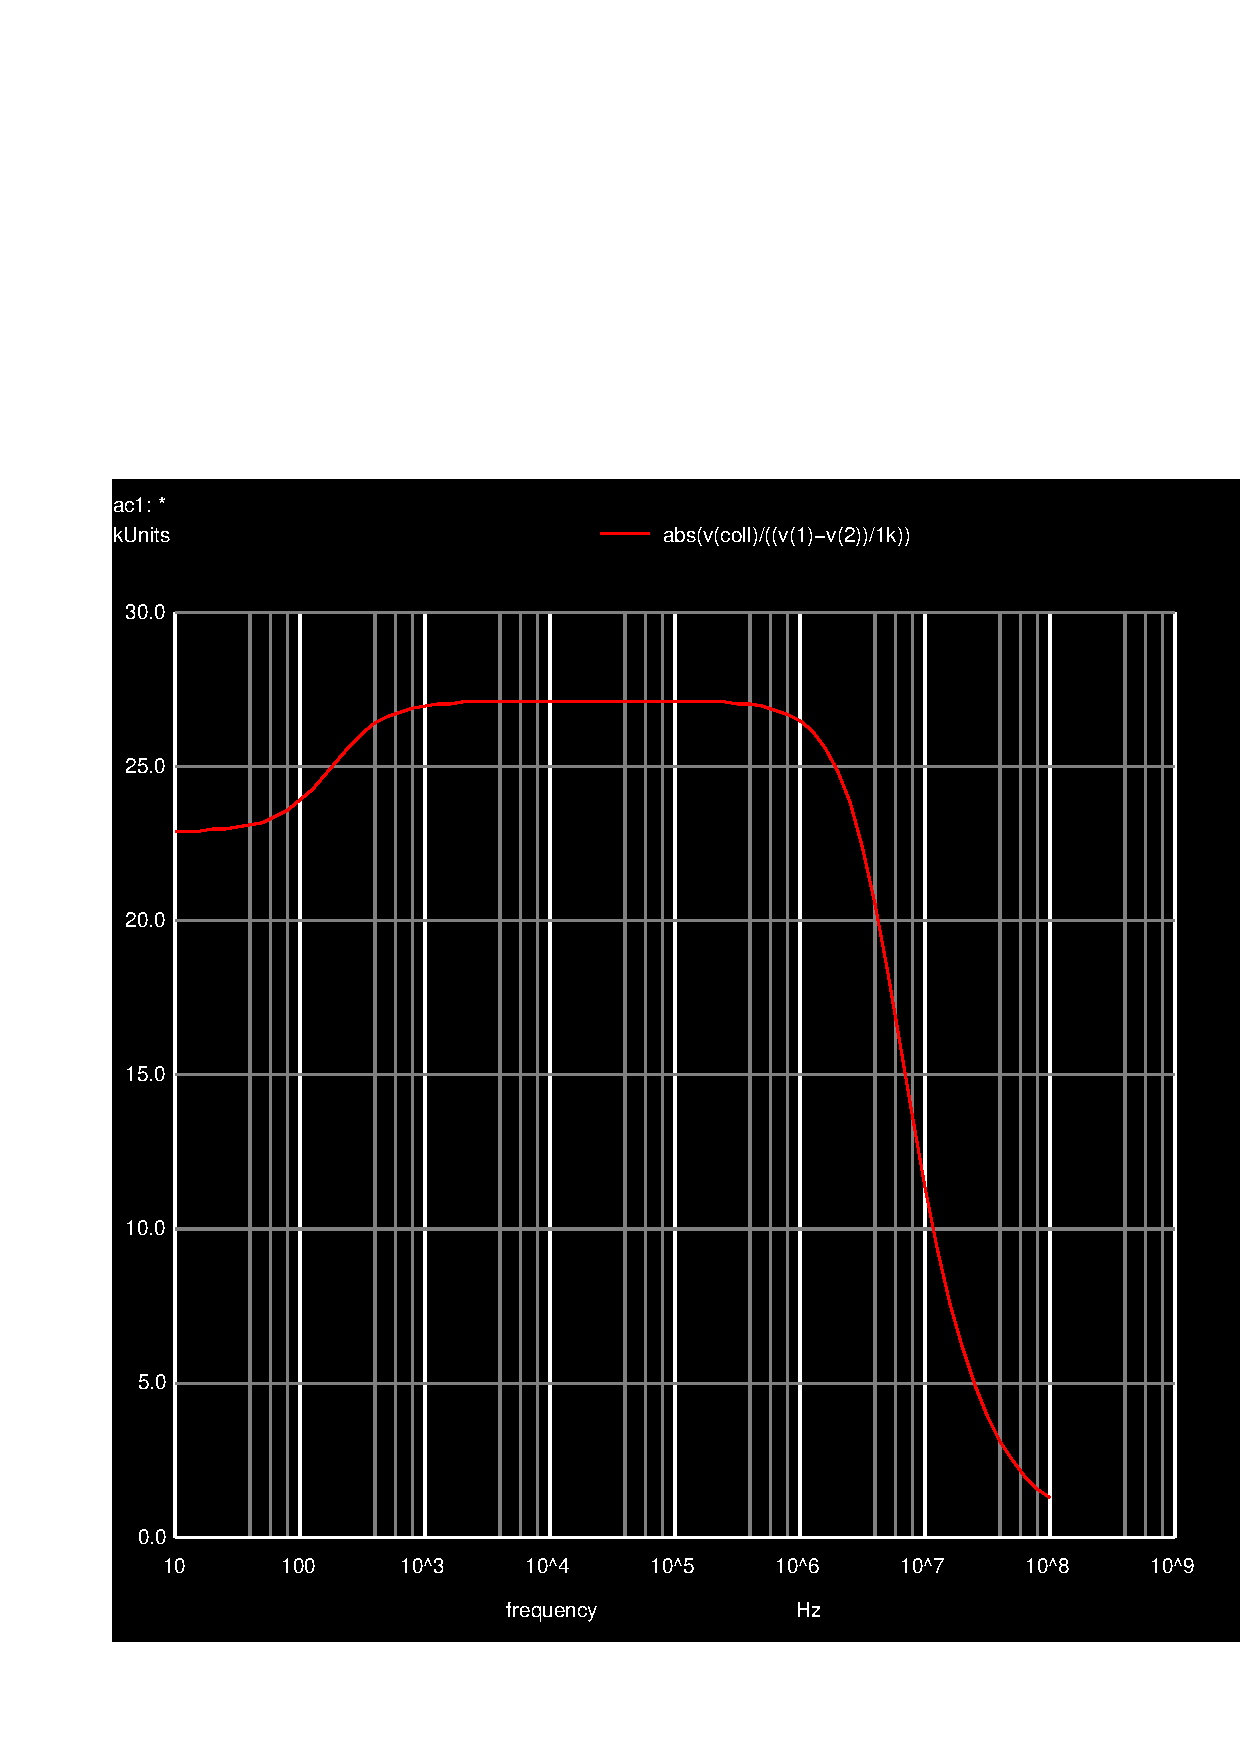
\includegraphics[width=0.6\linewidth]{zim.pdf}
\caption{Input impedance}
\label{fig:zim}
\end{figure}

\lipsum[1-1]





\section{Conclusion}
\label{sec:conclusion}


\par Unlike previous laboratories, this time, the results were not equal.

However, we believe that the differences are not that significant and they can be explained by how NGSpice solves the circuit compared to how it was done in the theoretical analysis.

To solve the circuit, NGSpice used far more advanced simulation methods for the diodes, with many more parameters, while we used an approximated model with $V_{on}$ and an incremental resistor. 

This way, the objective should have never been to have equal results, but rather, have results that are "close enough", which we believe it was achieved.


%To sum up, we believe that the goals of this report were achieved.

%\cleardoublepage

% ----------------------------------------------------------------------
%  Bibliography
% ----------------------------------------------------------------------
%\addcontentsline{toc}{section}{\bibname}
%\bibliographystyle{abbrvunsrtnat} % <<<<< SELECT IF USING REFERENCES BY NUMBER (CITATION ORDER)
%\bibliography{../../../BIBfile.bib}

% ----------------------------------------------------------------------
\end{document}
% ----------------------------------------------------------------------